\documentclass{article}


\usepackage[letterpaper, margin=0.70in]{geometry}
\usepackage{hyperref}
\usepackage{array, booktabs, siunitx}
\usepackage{fancyhdr}
\usepackage{listings}
\usepackage{xcolor}
\usepackage{tabularx}
\usepackage{natbib}

\usepackage{graphicx}
\usepackage{subcaption}

\usepackage{titlesec}
\titlespacing*{\section}
{0pt}{0.1in}{0.1in}

\titleformat{\section}
  {\normalfont\large\bfseries}  % subsection size
  {\thesection}{1em}{}

\titleformat{\subsection}
  {\normalfont\normalsize\bfseries}  % subsection size
  {\thesubsection}{1em}{}

\date{}
\headsep=0.15in
\pagestyle{fancy}
\fancyhf{}

\fancyhead[L]{ECEN-689}
\fancyhead[C]{Homework 2: VLMs}
\fancyhead[R]{Brody Jordan}

\lstset{language=Python}

\usepackage{titlesec}

\begin{document}

\noindent I evaluated two models: Qwen2.5-VL-3B-Instruct \citep{qwen} and ChatGPT 5.4 \citep{chatgpt}, with the ScanNet \citep{scannet} dataset, and looked at two specific VSTI-Bench \citep{visitbench} tasks: \verb|camera_movement_direction| and \verb|camera_obj_abs_dist|.

\begin{table}[h]
    \centering
    \caption{Aggregate Model Performance Comparison}
    \vspace*{-0.1in}
    \label{tab:combined_results}
    \begin{tabular}{@{}llcc@{}}
        \toprule
        \textbf{Model} & \textbf{Task Category} & \textbf{Metric} & \textbf{Score} \\ \midrule
        Qwen2.5-VL     & Camera Movement        & ACC             & 31.9\%         \\
                       & Absolute Distance      & MRA             & 0.68           \\ \midrule
        ChatGPT 5.4    & Camera Movement        & ACC             & 36.6\%         \\
                       & Absolute Distance      & MRA             & 0.63           \\ \bottomrule
    \end{tabular}
\end{table}
Now an example failure:
\begin{figure}[h!]
    \centering
    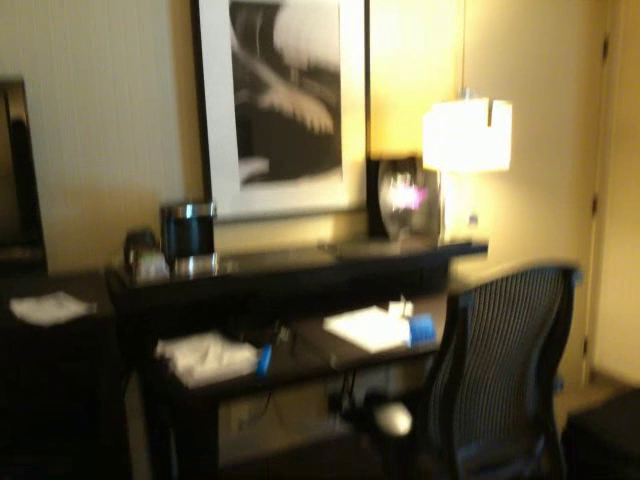
\includegraphics[width=0.5\linewidth]{frame26.png}
    \caption{VSTI-Bench Task 1975}
    \label{fig:movement}
    % \begin{subfigure}{0.45\textwidth}
    %     \includegraphics[width=\linewidth]{absolute_distance.png}
    %     \caption{Camera Object Absolute Distance Task}
    %     \label{fig:distance}
    % \end{subfigure}
\end{figure}
Here the ground truth is 1.1, but Qwen2.5-VL estimated it to be 1.8 meters and ChatGPT 5.4 estimated it to be 2.0 meters. \\

\noindent The primary failure modes expose a fundamental architectural limitation: VLMs struggle to infer rigid 3D geometry purely from 2D pixel patches. \\

\begin{thebibliography}{9}
    \bibitem[Dai et al.(2017)]{scannet}
    A. Dai et al., ``ScanNet: Richly-annotated 3D Reconstructions of Indoor Scenes,'' \textit{Proc. CVPR}, 2017.

    \bibitem[Qwen Team(2025)]{qwen}
    Qwen Team, ``Qwen2.5-VL Technical Report,'' \textit{arXiv:2502.13923}, 2025.

    \bibitem[OpenAI(2026)]{chatgpt}
    OpenAI, ``ChatGPT (Version 5.4),'' \textit{OpenAI Blog}, 2026.

    \bibitem[Bitton et al.(2023)]{visitbench}
    Y. Bitton et al., ``VisIT-Bench: A Benchmark for Vision-Language Instruction Following,'' \textit{Proc. NeurIPS}, 2023.
\end{thebibliography}



\end{document}

